\section{OpenGeoSys - Finite-Element-Method}
\label{app:ogs}

\begin{wrapfigure}{l}{6cm}
  \centering
  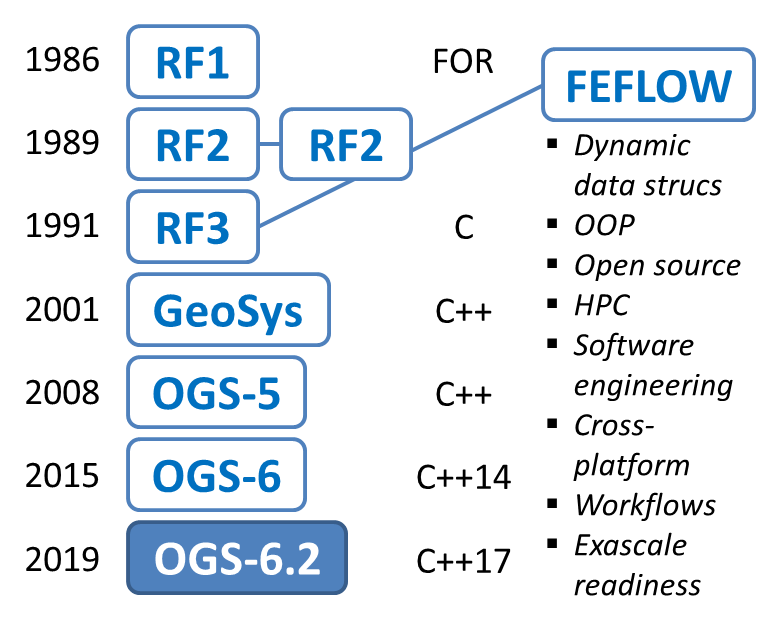
\includegraphics[width=6cm]{figures/ogs-2019}
  \caption{OpenGeoSys development history}
  \label{fig:ogs-history}
\end{wrapfigure}
OpenGeoSys (OGS) is a scientific open-source initiative for the numerical simulation of thermo-hydro-mechanical/chemical (THMC) processes in porous and fractured media, inspired by FEFLOW \cite{Diersch2014} and ROCKFLOW concepts and continuously developed since the mid-eighties (Fig. \ref{fig:ogs-history}), see e.g. \cite{Kolditz:1990}, \cite{Wollrath:1990}, \cite{Kroehn:1991} and \cite{Helmig:1993}. Meanwhile, more than 50 PhD projects have been dedicated to the OGS development since the merger in the nineties.

The OGS framework is targeting applications of various disciplines in environmental geoscience, e.g., in the fields of regional \cite{Jing20181989}, contaminant \cite{Nixdorf2017598} and coastal hydrology \cite{Walther2017648}, fundamental geothermal processes \cite{Parisio2019} and geothermal energy systems \cite{Meng2018971,HEIN201680}.
%
OGS is applied for energy storage applications in technical systems such as concrete \cite{Miao2019977} or  zeolite-based heat storage \cite{Lehmann20191102} and natural systems such as salt caverns \cite{Bottcher2017,Nagel2017}. 
%
OGS is also used in fundamental studies for nuclear waste management \cite{Shao201933}.

The most recent version, OpenGeoSys-6 (OGS-6) \cite{Naumov:2018,Bilke2019}, is a complete re-implementation of the multi-physics code OpenGeoSys-4/5 \cite{Kolditz2004225,Wang:2006} using advanced methods in software engineering and architecture with a focus on code quality, modularity, performance and comprehensive documentation. The current release version OpenGeoSys 6.2.0 \cite{ogs:6.2.0} will be dedicated to analyze and predict the behaviour of geosystems becoming more and more relevant in future like nuclear waste deposition, geothermal use of subsurface resources for power and heat production, and geological storage of various energy carriers. Particular emphasis is put on the implementation of advanced numerical methods for the propagation of discontinuities, such as enriched finite element function spaces \cite{Watanabe2012}, non-local formulations \cite{Parisio2017} and phase-field models for fracture \cite{Yoshioka2019} with the ability to utilize HPC platforms~\cite{Wang2014a,Wang:2017}.

OpenGeoSys is participating in several international model development, validation and benchmarking initiatives, e.g., DEVOVALEX (with applications mainly in the assessment of waste repositories, see~\cite{Birkholzer2018}), CO2BENCH (geological CO\textsubscript{2} storage, see~\cite{Kolditz2012613}), SeS Bench (reactive transport processes, see~\cite{Steefel:2015}) and HM-Intercomp (coupled hydrosystems, see~\cite{Maxwell:2015}).

The OGS community provides an ongoing series of benchmark books \cite{BB4} and tutorials \cite{Lehmann:2018}. For more information please refer to the OpenGeoSys webpage \url{www.opengeosys.org}.